\documentclass[12pt, letterpaper]{article}
\usepackage{graphicx} % Required for inserting images
\usepackage{fancyhdr}
\usepackage{placeins}
\usepackage[hidelinks]{hyperref}
\pagestyle{fancy}
\title{Final Assignment:

Integration of Tools and Practices
}
\author{Mani Sazvar}
\date{dey month of 4031 semester}
\begin{document}
\maketitle
\begin{center}
Github repository:

\url{https://github.com/mani-the-great/cw_final}
\end{center}
\thispagestyle{empty}
\newpage
\pagenumbering{arabic} 
\tableofcontents
\newpage
\section{Git and Github}
\subsection{Repository Initialization and Commits}
First, I created a new repository on github and named it as cw\_final.
then I created a new file on my laptop and cloned the recently created repository in it. To do so I opened powershell and typed: "git clone https://github.com/mani-the-great/cw\_final.git"
\subsection{ GitHub Actions for LaTeX Compilation
}
In my repository I clicked on the "Action" tab and then I clicked on "New workflow button".

I opened the link provdided on the PDF( TA's repository) and copied the contents of the main.yml file and pasted it in my own main.yml file.
\section{Exploration Tasks}
\subsection{Vim Advanced Features}
\begin{enumerate}
    \item \textbf{Registers for Advanced Clipboard Management}: Vim provides a powerful clipboard management system through registers. Registers let you store and retrieve text for reuse, including yanked text, macros, and more.Key Registers:
    
    "": Default unnamed register (last yanked/deleted text).
    
    "0: Yank register (stores the last yanked text).
    
    "1 to "9: Delete registers (store the last nine deletions).
    
    "a to "z: Named registers for custom storage.
    
    "+ : System clipboard register (for copy-pasting outside Vim).
    
    \textbf{use case}: allows selective pasting and better organization of copied text for complex editing workflows.

    \item \textbf{Macros for automating repetitive tasks}: Macros in vim are a way to record a sequnce of commands. this feature is useful for automating repetitive edits.

    \textbf{Use case}: for talks like reforming code, editing structured data, or applying the same change across multiple lines.
    \item \textbf{Custom key mapping for efficiency}: Vim allows you to create custom key mapping to strreamline your workflow and execute complex commands with a single keystroke.

    \textbf{how to create mapping}:

    \begin{itemize}
  \item Use :map for normal mode mappings.
  \item Use :imap for insert mode mappings.
  \item Use :vmap for visual mode mappings.
\end{itemize}

    \textbf{Use case}: reduces keystrokes for frequent actions and enables customization of vim to fit your workflow.
\subsection{Memory profiling}
\subsubsection{Memory leak}
\textbf{what is a Memory Leak?} A memory leak occurs when a program allocates memory but fails to release it after it's no longer needed. Over time, this can lead to a gradual consumption of memory resources, eventually slowing down or crashing the system due to insufficient memory.

\textbf{How Memory Leaks Can Occur?} Memory leaks are often caused by programming mistakes or improper resource management. Here are common ways they can occur:

\begin{itemize}
    \item Failure to free dynamivally allocated memory
    \item Retaining refrences in garbage collecting languages like java or python
    \item Global or static variables(because of their lifetime persisting for the duration of the program)
\end{itemize}
\subsubsection{Memory profilers}
\textbf{what is Valgrind?}Valgrind is a powerful programming tool primarily used for memory debugging, memory leak detection, and profiling in C, C , and other languages. It helps developers identify and fix issues related to memory allocation, deallocation, and usage.Valgrind operates by running programs in a controlled environment, analyzing how memory is being used and reporting issues such as:
memory leaks - use of uninitialized memory - accessing memory outside allocated bounds, etc.
\textbf{what does valgrind do when a memory leak happens?} It reports detailed information about the issue.for example:
\begin{itemize}
    \item leaked blocks: it showshow many blocks of memory were allocated but not freed.
    \item bytes lost: the amount of memory(in bytes) that were leaked.
    \item leak type: valgrind categorizes memory leaks into types.
\end{itemize}
\subsection{GNU/Linux Bash Scripting}
\subsubsection{fzf}
\begin{itemize}
    \item \textbf{What is Fuzzy Searching?}Fuzzy searching is a technique that allows you to find approximate matches for a query, rather than requiring an exact match. It is particularly useful when working with large datasets or filenames, where users may not remember the exact string or want to type the entire name.
    
    \textbf{How Does Fuzzy Searching Work in the Context of FZF?}FZF (Fuzzy Finder) is a command-line tool that uses fuzzy searching to let users interactively search and filter lists. It does this by ranking potential matches based on how closely they align with the query, often using scoring algorithms.
    \item \textbf{The command "ls $|$ fzf" does the following}:
    \begin{enumerate}
        \item ls: lists the files and directories in the current directory. produces a plain list of names as output.

        \item Pipe($|$): passes the output of ls(the list of files and directories) to the next command, fzf.

        \item fzf: opens an interactive fuzzy finder interface. It displays the list of files and directories by ls. Allows you to search for a specific name using fuzzy matching rules.
    \end{enumerate}
    \end{itemize}
\subsubsection{Using fzf to find your favorite PDF}
\begin{enumerate}
    \item fd -e pdf
    \item fd -e pdf $|$ fzf
\end{enumerate}
\subsubsection{Opening the file using Zathura}
zathura "\$( fd -e pdf $|$ fzf)"
\section{Git and FOSS}
\subsection{README.md} I created the readme file. it is available on the repository.
\subsection{Issues}
\begin{figure*}[!b]
    \centering
    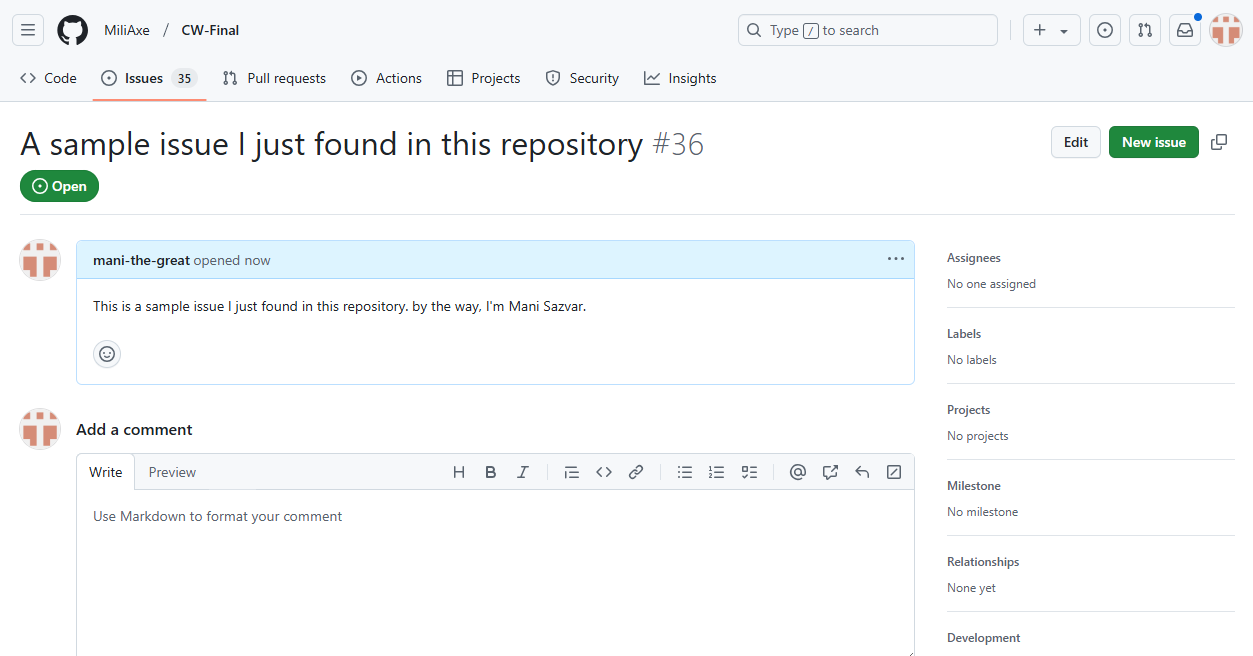
\includegraphics[width=1\linewidth]{ggvg.png}
    \caption{This is a sample issue i created}
    \label{fig:enter-label}
\end{figure*}
\FloatBarrier

\subsection{FOSS contribution}
Yes, I like to contribute to FOSS projects. At first I didn't know anything about it. but when I realized its importance, I got motivated to contribute to it. The type of projects that I mostly like to contribute are general-use softwares like linux or libreoffice. I also think that contributing to these kinds of software will be a good resume for a software engineer. 
\end{enumerate}
\end{document}
